\chapter{Recurrent neural networks (RNN)}\label{ch-20}

This is a light introduction to \textbf{recurrent neural networks}
(RNNs), which will be studied in depth in the ISPR and CNS courses. So
far networks were \textbf{feedforward} (input → output direction) and
worked on \textbf{vectors}. RNNs add \textbf{feedback connections}
(cycles) to the topology: the presence of self-connections gives the
network \textbf{dynamic properties} and a \textbf{memory} (a state) of
past computations. This extends the representational capacity of the
model to the processing of \textbf{sequences} (and structured data).
RNNs are also biologically plausible: biological neural networks are
recurrent.

\section{Why sequential data}\label{perchuxe9-i-dati-sequenziali}

Models for sequences are needed when the output depends on the
\textbf{history of the inputs} (for example over time: dynamic models),
or when the domain consists of \textbf{variable-length sequences}:

\begin{itemize}
\tightlist
\item
  dynamic processes, signal processing (filters, control), robotics;
\item
  \textbf{language}: speech recognition, NLP, formal languages,
  information retrieval;
\item
  vision and reasoning about temporal events;
\item
  \textbf{time series}: financial forecasting, signal processing;
\item
  genomics and proteomics (bioinformatics): for example predicting the
  structure of a protein from its amino acid sequence;
\item
  human activity recognition from sensor data.
\end{itemize}

RNNs (and related approaches) have been the reference for sequence
processing, with state-of-the-art results in \textbf{speech
recognition} and \textbf{text processing} (machine translation\ldots),
but also for ``fun'' applications such as music composition and text
and speech generation.

\section{From flat data to structured
data}\label{dai-dati-piatti-ai-dati-strutturati}

So far data were \textbf{flat} (vectors). \textbf{Structured} data are
sequences, trees, graphs, multi-relational data: strings, proteins,
time series, small molecules, networks.

\subsection{The new domain: sequences and
transductions}\label{il-nuovo-dominio-sequenze-e-trasduzioni}

\begin{itemize}
\tightlist
\item
  \textbf{Data}: discrete sequences of \textbf{vectors} (with a serial
  order, for example time), of variable length. Each element
  \(\mathbf{l}_t\) is a vector (e.g.\ \(\mathbf{l}_t = [1, 0, 1, 0.7]\)).
\item
  \textbf{Task}: a \textbf{transduction} in the sequential domain,
  i.e.\ a mapping \emph{input sequence → output value or sequence}.
\end{itemize}

\begin{figure}[htbp]
\centering
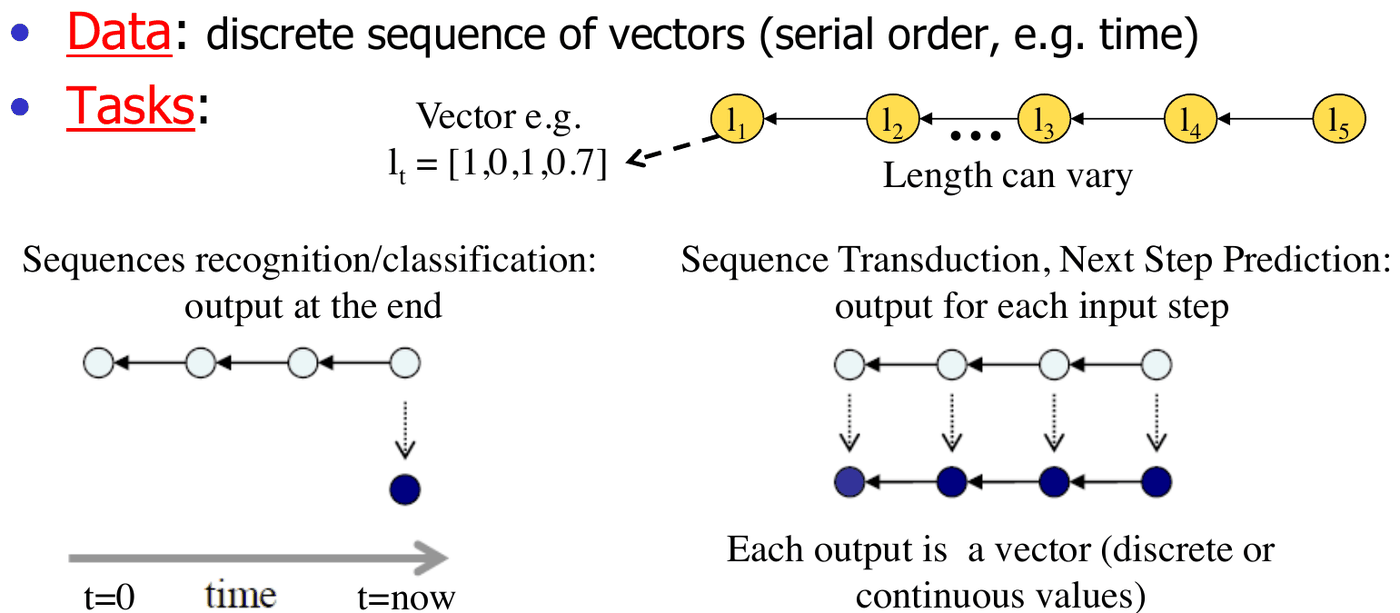
\includegraphics[width=0.80\linewidth,height=0.42\textheight,keepaspectratio]{images/20-rnn_trasduzioni.png}
\caption{Sequence recognition/classification (output at the end) and
sequence transduction (output at each step).}
\end{figure}

\begin{figure}[htbp]
\centering
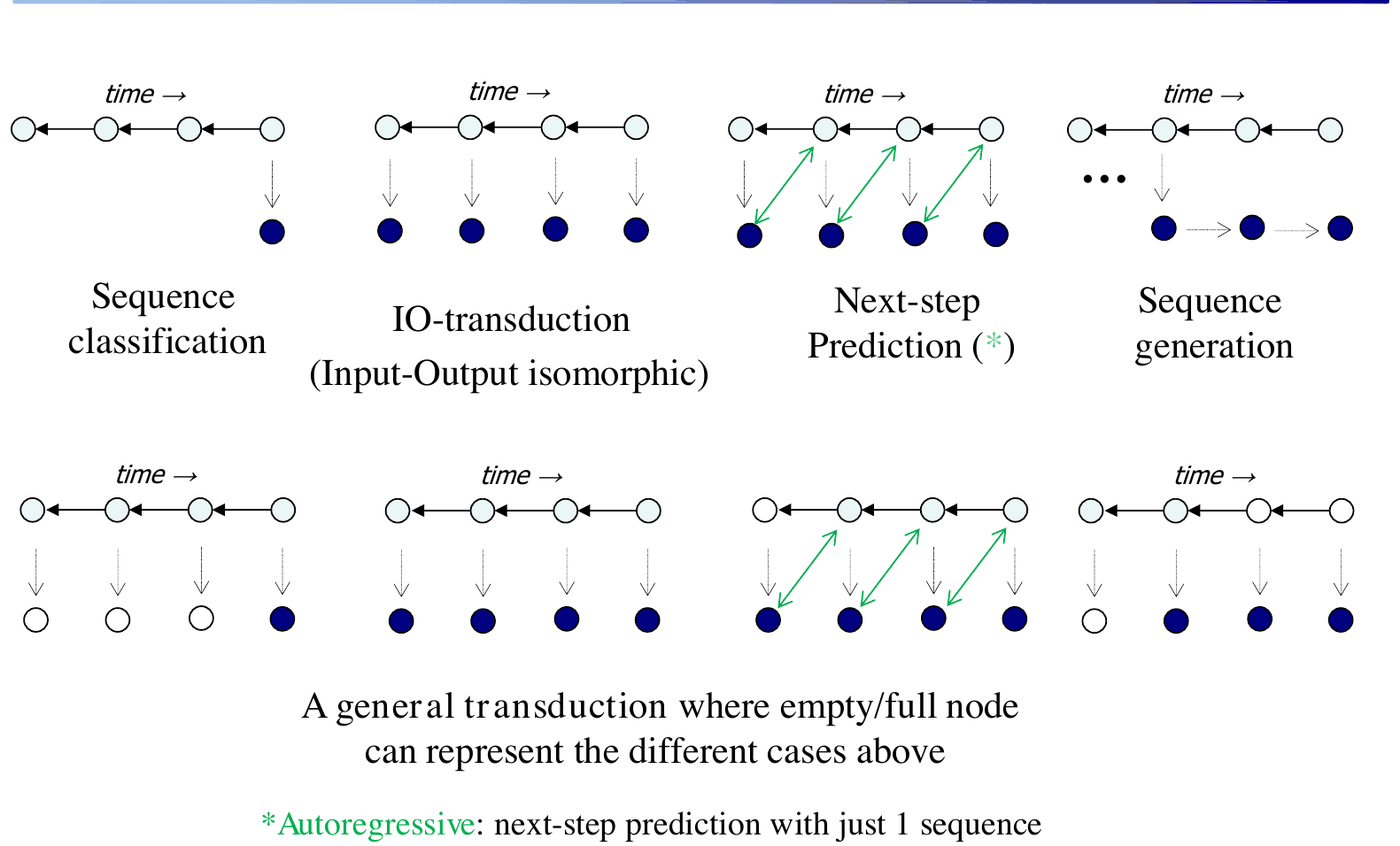
\includegraphics[width=0.80\linewidth,height=0.42\textheight,keepaspectratio]{images/20-rnn_tipi-trasduzione.png}
\caption{Types of transduction: sequence classification, isomorphic IO
transduction (one output per input), next-step prediction, sequence
generation. Autoregressive prediction uses a single sequence.}
\end{figure}

\section{Memory in neural
networks}\label{la-memoria-nelle-reti-neurali}

The goal is for the output to depend on \textbf{previous} inputs.

\subsection{Approach 1: finite memory
(IDNN)}\label{approccio-1-memoria-finita-idnn}

The first approach is ``spatial'', with \textbf{finite memory}:
\textbf{Input Delay Neural Networks} (in the class of \emph{Time-Delay
NNs}, already seen at the beginning of CNNs). The delays are in the
connections and act as a memory of the input: a finite-size
\textbf{shift register}, a \textbf{sliding window} over the sequence.
(CNNs extended this idea to 2D images.)

\begin{figure}[htbp]
\centering
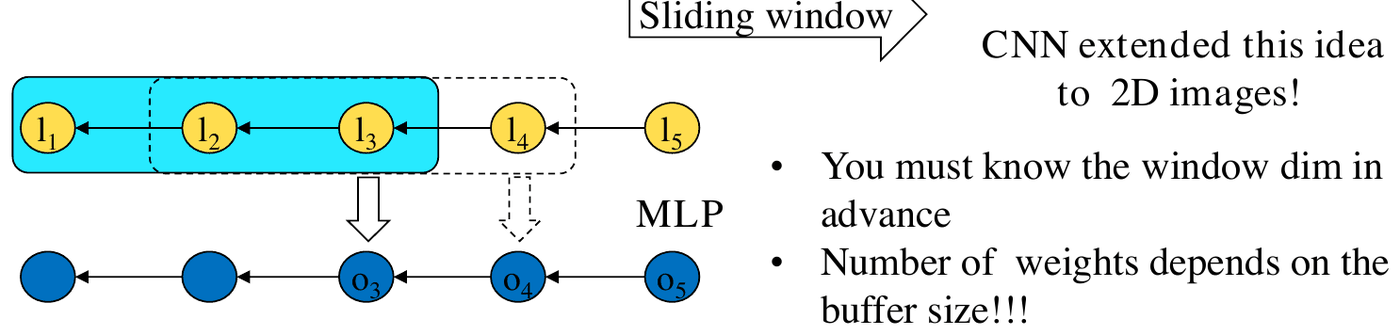
\includegraphics[width=0.74\linewidth,height=0.42\textheight,keepaspectratio]{images/20-rnn_idnn.png}
\caption{IDNN: a fixed-size sliding window over the sequence, processed
by an MLP.}
\end{figure}

\begin{itemize}
\tightlist
\item
  The window size must be \textbf{known in advance}.
\item
  The number of weights \textbf{depends on the buffer size}.
\item
  If the buffer contains enough information, the problem is solved with
  normal MLP training (for example NETtalk, 1988).
\end{itemize}

\subsection{Approach 2: recurrent
units}\label{approccio-2-unituxe0-ricorrenti}

A \textbf{recurrent neural unit} has a feedback connection (a
\emph{self-loop}) and uses both the current input and the
\textbf{state} information: \[
x(t) = \tau\big(\mathbf{l}(t), x(t-1)\big) = f\big(\mathbf{w}^T\mathbf{l}(t) + \hat{w}\,x(t-1) + \theta\big), \qquad x(0) = 0,
\] where \(\mathbf{l}(t)\) is the input (label) at time \(t\), \(f\) is
the (sigmoidal) activation, \(\hat{w}\) is the \textbf{recurrent
weight}, \(\theta\) the bias, and \(x(t-1)\) is the state at the
previous step, provided by a unit delay \(q^{-1}\). The new part
compared to an ordinary neuron is the term \(\hat{w}\,x(t-1)\).

\begin{figure}[htbp]
\centering
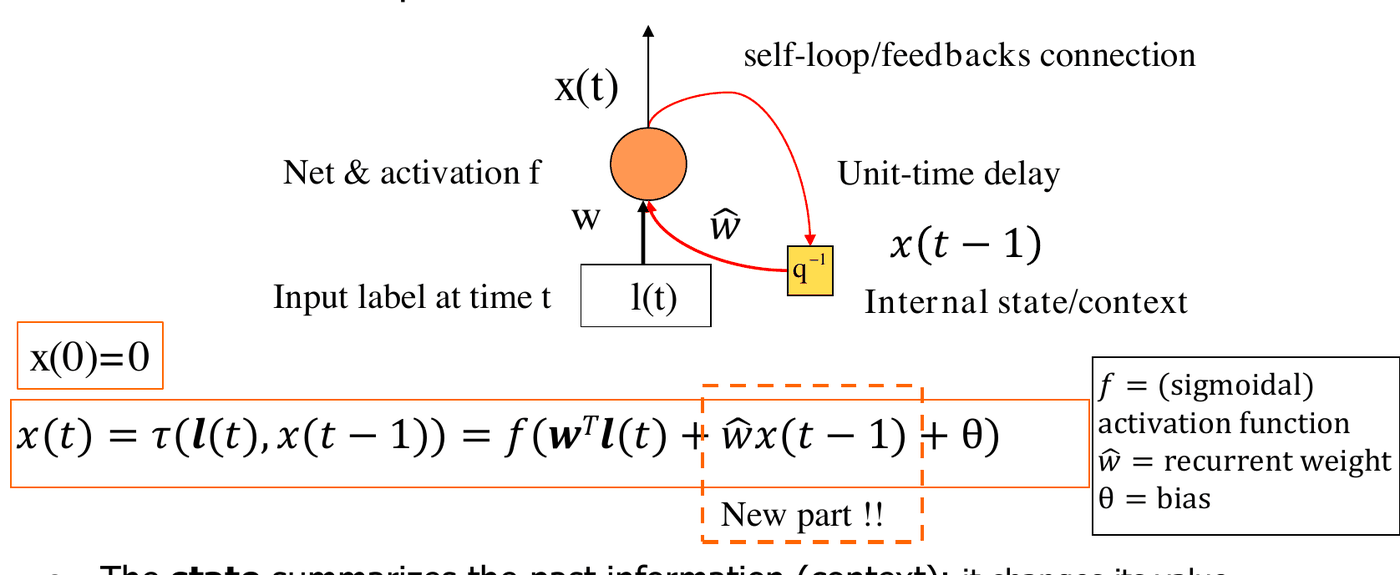
\includegraphics[width=0.86\linewidth,height=0.42\textheight,keepaspectratio]{images/20-rnn_unita-ricorrente.png}
\caption{A recurrent unit: the self-loop with unit delay brings the
previous state as an additional input.}
\end{figure}

\begin{itemize}
\tightlist
\item
  The \textbf{state} summarises past information (the
  \textbf{context}): it changes value following the flow of inputs.
\item
  The \textbf{encoding of the past is adaptive}, because it depends on
  the free weights of the model.
\end{itemize}

\begin{boxexample}{Exercise: counting the ``1''s}

Build an RNN with a single unit (finding the values of \(w\) and
\(\hat w\)) that returns the number of ``1''s received so far in a
sequence of 0s and 1s.

\textbf{Solution}: a linear unit with \(w = 1\), \(\hat w = 1\),
\(\theta = 0\), i.e.\ \(x(t) = l(t) + x(t-1)\). With input
\(1, 0, 1, 1, 0, 1\) the state is \(1, 1, 2, 3, 3, 4\): \textbf{the
state accumulates the sum of the ``1''s} received. The RNN summarises
the information of the past sub-sequence, something an IDNN
\textbf{cannot do} for variable-length sequences (its memory is limited
to the window).

\end{boxexample}

\subsection{State transition
systems}\label{sistemi-a-transizione-di-stato}

In general, a recurrent model is a \textbf{state transition system}: \[
\begin{cases} \mathbf{x}(t) = \tau\big(\mathbf{x}(t-1), \mathbf{l}(t)\big) \\ \mathbf{y}(t) = g\big(\mathbf{x}(t), \mathbf{l}(t)\big) \end{cases} \qquad \mathbf{x}(0) = \mathbf{0}.
\]

\begin{figure}[htbp]
\centering
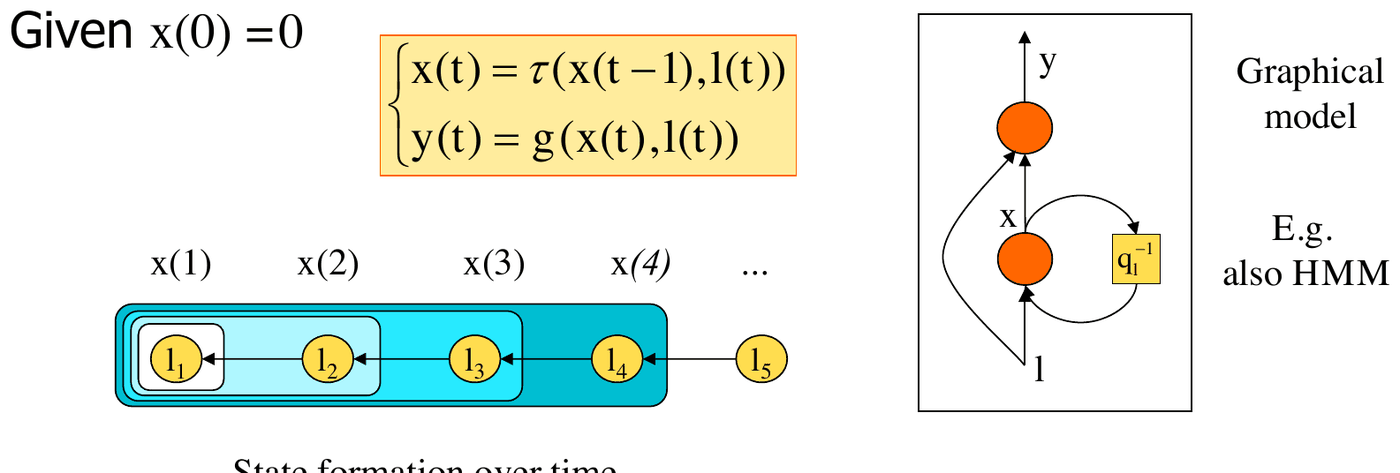
\includegraphics[width=0.80\linewidth,height=0.42\textheight,keepaspectratio]{images/20-rnn_sistema-stati.png}
\caption{State transition system: the state at time \(t\) encodes the
past sub-sequence.}
\end{figure}

\begin{itemize}
\tightlist
\item
  \(\tau\) is the \textbf{state transition function} (\emph{next-state
  function}), implemented by a neural network.
\item
  The state summarises past inputs: it is an \textbf{encoding}
  (embedding) of the sub-sequences.
\item
  The state has \textbf{continuous} (real) values (unlike, for example,
  automata or HMMs, which have discrete states).
\item
  \(\mathbf{x}(t)\) can be a set of states, to compose a network of
  recurrent units.
\end{itemize}

\subsection{A recurrent network (Simple
RNN)}\label{una-rete-ricorrente-simple-rnn}

With many hidden recurrent units we obtain Elman's \textbf{Simple
RNN}: each hidden unit receives the input and the previous states of
\textbf{all} hidden units (through the delays), and an (optional)
output layer produces \(\mathbf{y}(t)\).

\begin{figure}[htbp]
\centering
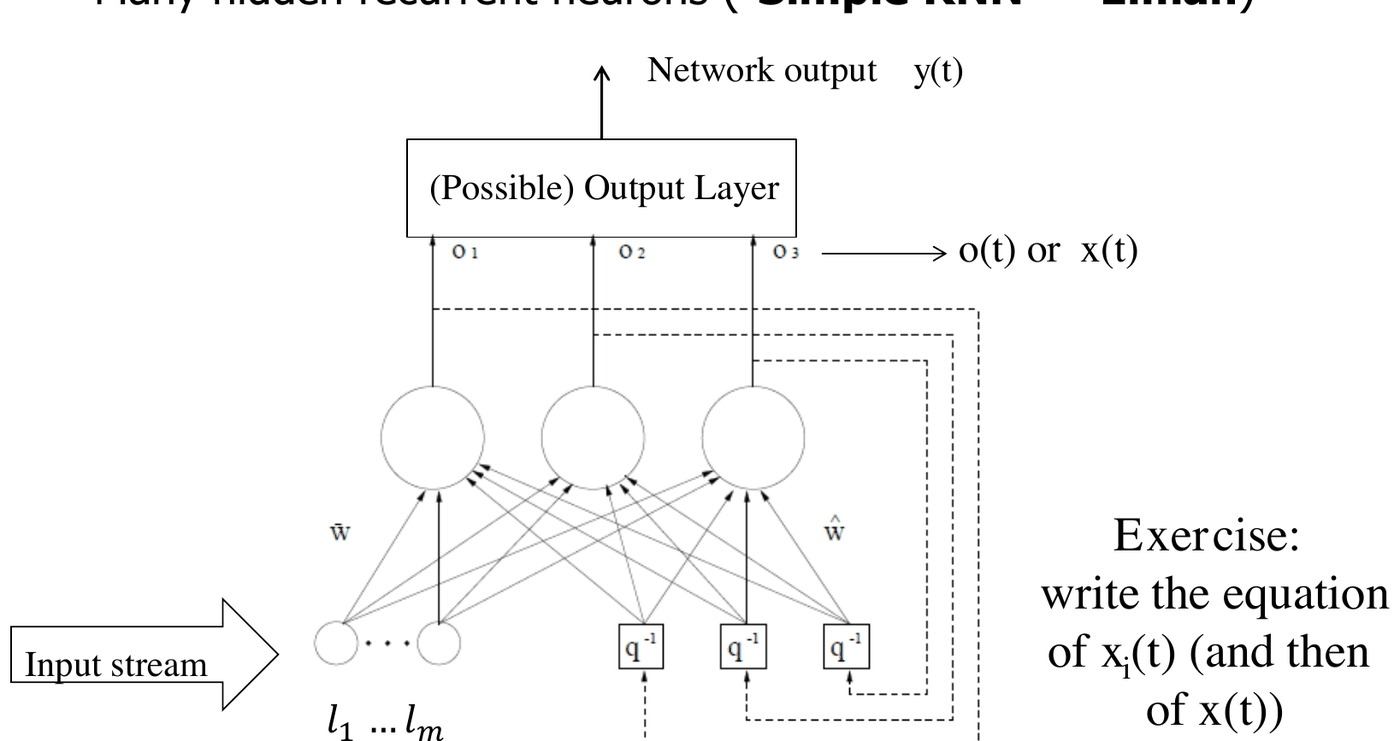
\includegraphics[width=0.86\linewidth,height=0.42\textheight,keepaspectratio]{images/20-rnn_elman.png}
\caption{A Simple RNN (Elman) with several hidden recurrent units.}
\end{figure}

\begin{boxexample}{Exercise: the equations}

For hidden unit \(i\): \[
x_i(t) = f\left(\sum_{j=1}^{m} w_{ij}\,l_j(t) + \sum_{k} \hat w_{ik}\,x_k(t-1) + \theta_i\right),
\] and in vector form
\(\mathbf{x}(t) = f\big(W\mathbf{l}(t) + \hat W\mathbf{x}(t-1) + \boldsymbol{\theta}\big)\).

\end{boxexample}

\subsection{Properties}\label{proprietuxe0}

Even the simple RNN is already very powerful:

\begin{itemize}
\tightlist
\item
  it is a \textbf{universal approximator} of non-linear dynamical
  systems;
\item
  it is \textbf{Turing-equivalent} (it can simulate any automaton);
\item
  it is a (non-autonomous) non-linear dynamical system, which can be
  studied with dynamical systems theory (chaos, fractals\ldots).
\end{itemize}

Recurrent models rest on three assumptions:

\begin{itemize}
\tightlist
\item
  \textbf{Causality}: the output at time \(t_0\) depends only on the
  inputs at times \(t \le t_0\). It is necessary and sufficient for
  having an internal state.
\item
  \textbf{Stationarity}: time invariance (after training): the
  transition function \(\tau\) is \textbf{the same} at every instant,
  regardless of the length of the sequences. This is what makes it
  possible to process variable-length data with a fixed-size model.
\item
  \textbf{Adaptivity}: the transition functions are implemented by
  neural networks with free weights, hence \textbf{learned from data}.
\end{itemize}

\section{Learning: unfolding}\label{apprendimento-lunfolding}

The same model is \textbf{unfolded} in time along the input sequence: a
feedforward MLP (the \textbf{encoding network}) equivalent to the RNN
over the \(k\) steps of the sequence is built, with \textbf{a replica
of the model for each step}. By stationarity, the replicas
\textbf{share the weights}.

\begin{figure}[htbp]
\centering
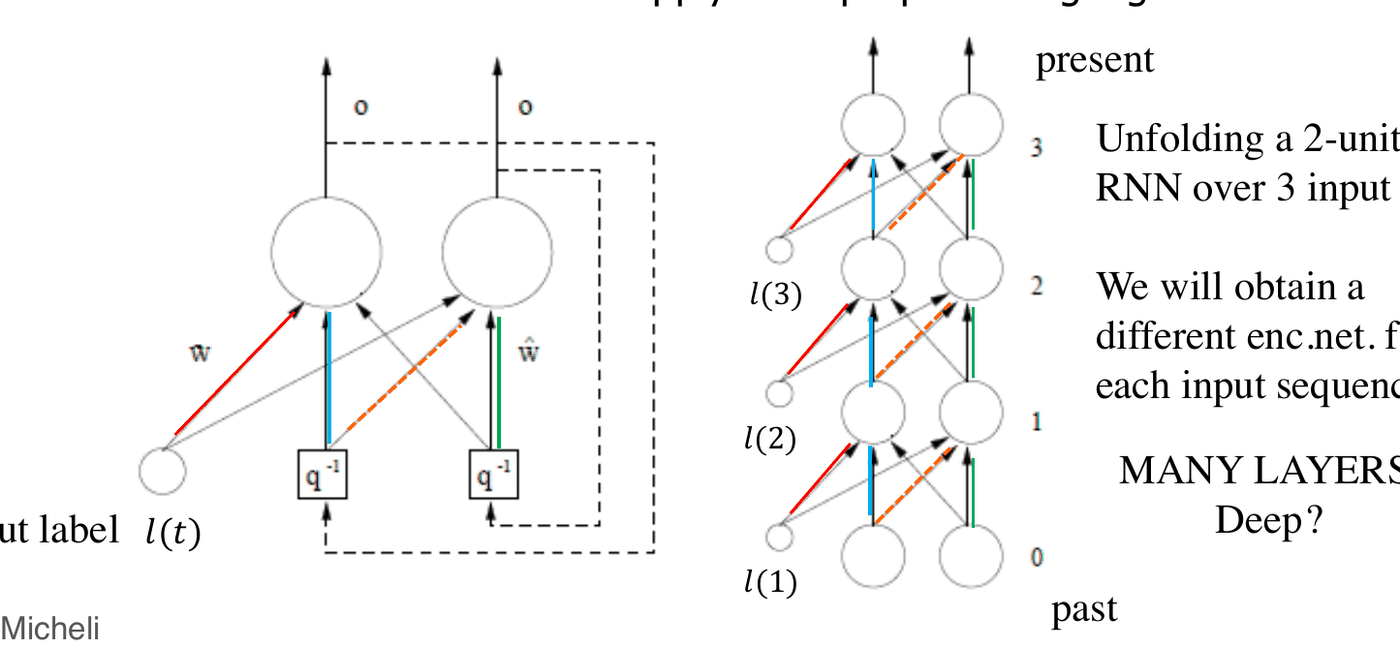
\includegraphics[width=0.74\linewidth,height=0.42\textheight,keepaspectratio]{images/20-rnn_unfolding.png}
\caption{Unfolding of a 2-unit RNN over 3 input steps: a many-layer
feedforward network is obtained, different for each input sequence.}
\end{figure}

\begin{boxtip}{The key point}

\textbf{Backpropagation} can be applied to the unfolded encoding
network! A different network is obtained for each input sequence, with
\textbf{many layers} (as many as the steps): it is de facto a
\textbf{deep} network, with weights shared across layers.

\end{boxtip}

Supervised learning algorithms for RNNs must take into account all the
encoding transitions developed by the model at each step:

\begin{itemize}
\tightlist
\item
  \textbf{BPTT} (\emph{Back-Propagation Through Time});
\item
  \textbf{RTRL} (\emph{Real-Time Recurrent Learning}).
\end{itemize}

They compute in different ways the same gradient of the output errors
on the equivalent unfolded network.

\begin{boxwarning}{Long-term dependencies}

Since the unfolded network is very deep, the \textbf{vanishing
gradient} makes it hard to learn \textbf{long-term dependencies} (when
the output depends on inputs very far in the past).

\end{boxwarning}

\subsection{Advanced models}\label{modelli-avanzati}

It is a rapidly growing research field, with many variants:

\begin{itemize}
\tightlist
\item
  \textbf{LSTM} (\emph{Long Short-Term Memory}): they try to solve the
  vanishing gradient with \textbf{``gate'' units} able to select the
  flow of the past and of the gradient. They were born for
  \textbf{long} dependencies: they are not suited to short series, so,
  despite their popularity, they should not be used uncritically;
\item
  \textbf{GRU} (\emph{Gated Recurrent Units}): a simplified LSTM;
\item
  \textbf{BRNN} (bidirectional RNNs): they consider both the left and
  the right context;
\item
  deep networks and RNNs are often merged;
\item
  against the vanishing gradient: Hessian-free optimisers, pre-training
  techniques\ldots{}
\end{itemize}

They are included in the main libraries (PyTorch, Keras,
Matlab\ldots). Some data on their spread: in 2015 LSTMs were used in 2
billion Android phones and 1 billion iPhones (Siri); in 2016 almost
30\% of the inference computing power of Google's datacentres was used
for LSTMs; in 2017 they were in Alexa and Facebook (30 billion
translations per week). A curious example: generating the
\textbf{handwritten} version of a text by predicting one \((x,y)\) point
of the pen trajectory at a time (Graves, 2013).

\section{Related approaches}\label{approcci-collegati}

\begin{itemize}
\tightlist
\item
  SOMs and unsupervised networks for sequential domains.
\item
  \textbf{Hidden Markov Models} (they model the probability
  distribution of state transitions).
\item
  \textbf{Transformers}.
\item
  \textbf{Randomised RNNs}: \textbf{Reservoir Computing} (ESN,
  \emph{Liquid State Machine}).
\item
  Distance-based models (string matching), string kernels, grammatical
  inference, ILP.
\end{itemize}

\subsection{Transformers and attention}\label{transformer-e-attenzione}

A \textbf{transformer} (2017) is a deep learning architecture based on
the parallel \textbf{multi-head attention} mechanism. Attention allows
the model to \textbf{access any previous point} of the sequence;
encoders and/or decoders plus feedforward networks complete the
architecture for different purposes.

The \textbf{attention layer} weighs all previous states according to a
\textbf{learned relevance} measure, potentially providing information
even about very distant tokens. It has proved particularly useful in
translation, where a distant context can be essential for the meaning
of a word. First used to improve RNNs, then also on its own
(\emph{``Attention is all you need''}). All tokens are processed
\textbf{simultaneously}, computing weights between their
representations (embeddings) in successive layers: they are simply
\textbf{scaled dot-product} units between \emph{query} vectors and word
vectors, which look for the highest correlations between the words of
a sentence (for example in ``see that girl'', ``that'' is associated
with ``girl''). It is also applied to image \emph{patches} instead of
words (\emph{vision transformer}).

\subsection{Randomised recurrent networks: Echo State
Networks}\label{reti-ricorrenti-randomizzate-le-echo-state-network}

Can we directly exploit this state machine to encode sequences, and
then use the resulting embedding to learn the output mapping? Yes,
\textbf{even with randomly connected recurrent networks with fixed}
(untrained) \textbf{weights}! This is the class of \textbf{Reservoir
Computing} (RC): Echo State Networks, \emph{liquid state machines},
\emph{fractal machines} (see
\href{18\%20-\%20Reti\%20neurali\%20randomizzate}{18 - Randomized
neural networks}).

\begin{figure}[htbp]
\centering
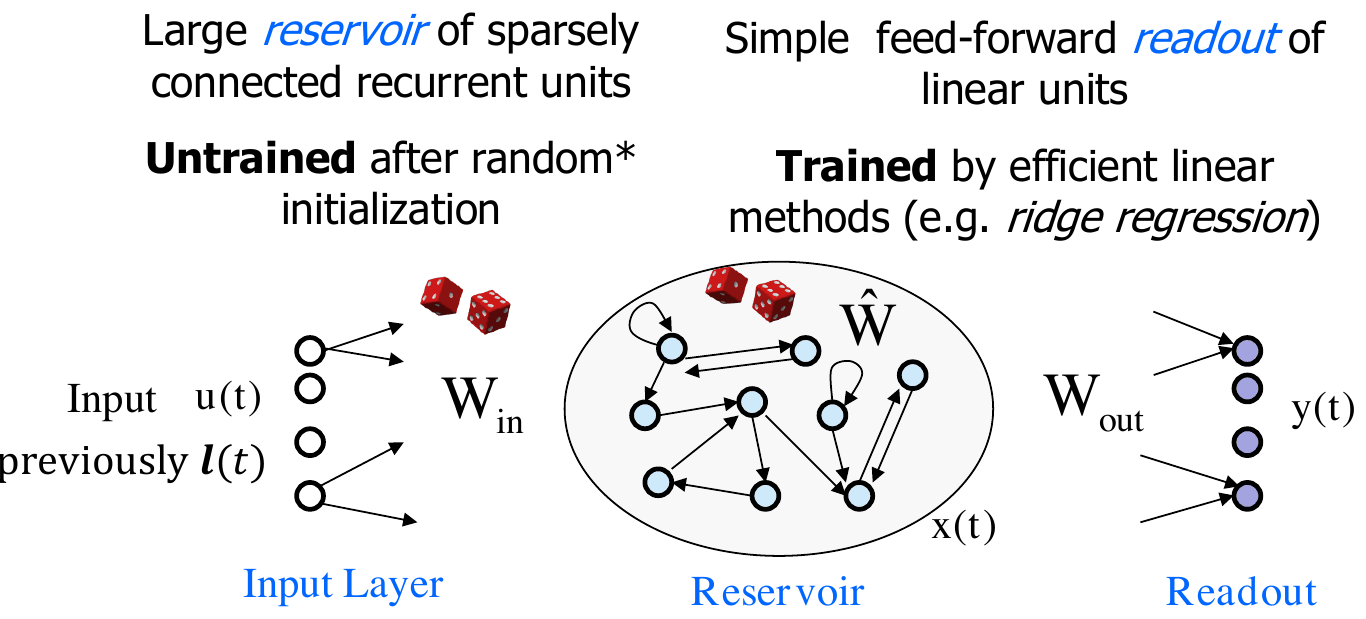
\includegraphics[width=0.80\linewidth,height=0.42\textheight,keepaspectratio]{images/20-rnn_esn.png}
\caption{An Echo State Network: untrained random reservoir and trained
linear readout.}
\end{figure}

\begin{boxdefinition}{Echo State Network (ESN)}

An ESN consists of: - a large \textbf{reservoir} of sparsely connected
recurrent units, \textbf{not trained} after a random initialisation; -
a simple feedforward \textbf{readout} of \textbf{linear} units, trained
with efficient linear methods (e.g.\ \textbf{ridge regression}).

\textbf{Echo State Property}: the state transition function must be
\textbf{contractive} (the spectral radius of the reservoir weights is
bounded, i.e.\ the stability of the dynamical system is guaranteed). In
this way the recurrent state depends asymptotically (like an
``echo'') \textbf{only on the input history}, and not on the initial
conditions of the state.

\end{boxdefinition}

ESNs are \textbf{very efficient} (no training of the recurrent units)
and solve tasks well under certain conditions.

\subsubsection{Markovian organisation of the state
space}\label{organizzazione-markoviana-dello-spazio-degli-stati}

\begin{figure}[htbp]
\centering
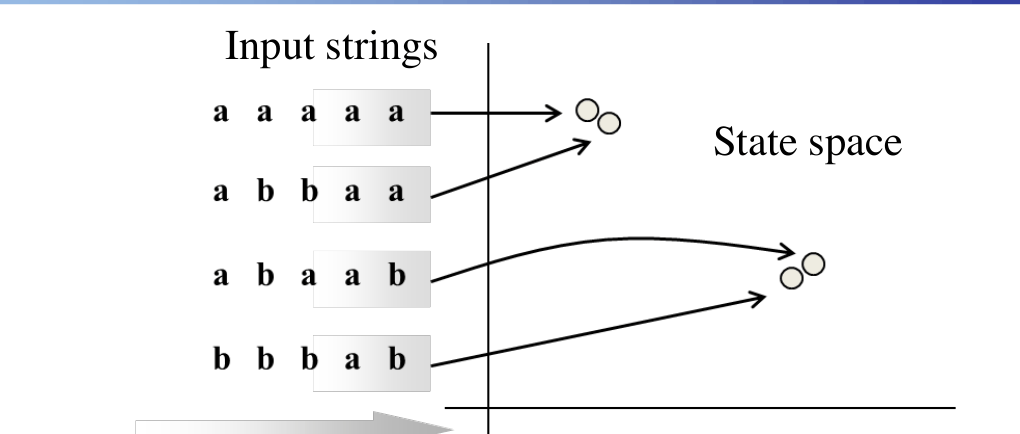
\includegraphics[width=0.54\linewidth,height=0.42\textheight,keepaspectratio]{images/20-rnn_markov.png}
\caption{The reservoir projects the sequences into the state space in a
``Markovian'' way: sequences with the same suffix end up close
together.}
\end{figure}

The reservoir acts as a \textbf{projection} (embedding) of the input
sequences into the state vector \(\mathbf{x}(t)\), and it is
intrinsically able to \textbf{discriminate sequences based on their
suffix}, without training the recurrent weights: the states are closer
the longer the \textbf{common suffix} (recent inputs matter more,
because of contractivity). This makes it easy to learn
\textbf{Markovian} tasks (also for trained RNNs, but ESNs are much more
efficient), and it is an \textbf{architectural bias} that also holds
for recurrent models with learning (Gallicchio, Micheli, 2011).

\textbf{Deep Reservoir Computing.} Several reservoirs can be stacked
(\textbf{DeepESN}, with many results from the CIML group in Pisa),
combining the power of deep RNNs with the efficiency of ESNs. The
layered organisation shows advantages in terms of \textbf{multiple time
scales} and \textbf{richness of dynamics}: in frequency analysis, the
higher layers focus on lower frequencies (wider time scales), forming a
hierarchical temporal representation.

\section{Towards structured domains}\label{verso-i-domini-strutturati}

Can the recurrent approach be extended to \textbf{trees}? Yes:
\textbf{recursive neural networks} (RecNN). Encoding proceeds
\textbf{bottom-up} (from the leaves to the root), and the state of each
vertex depends on its label and on the states of its
\textbf{children} (extending the transition function to several
states).

\begin{figure}[htbp]
\centering
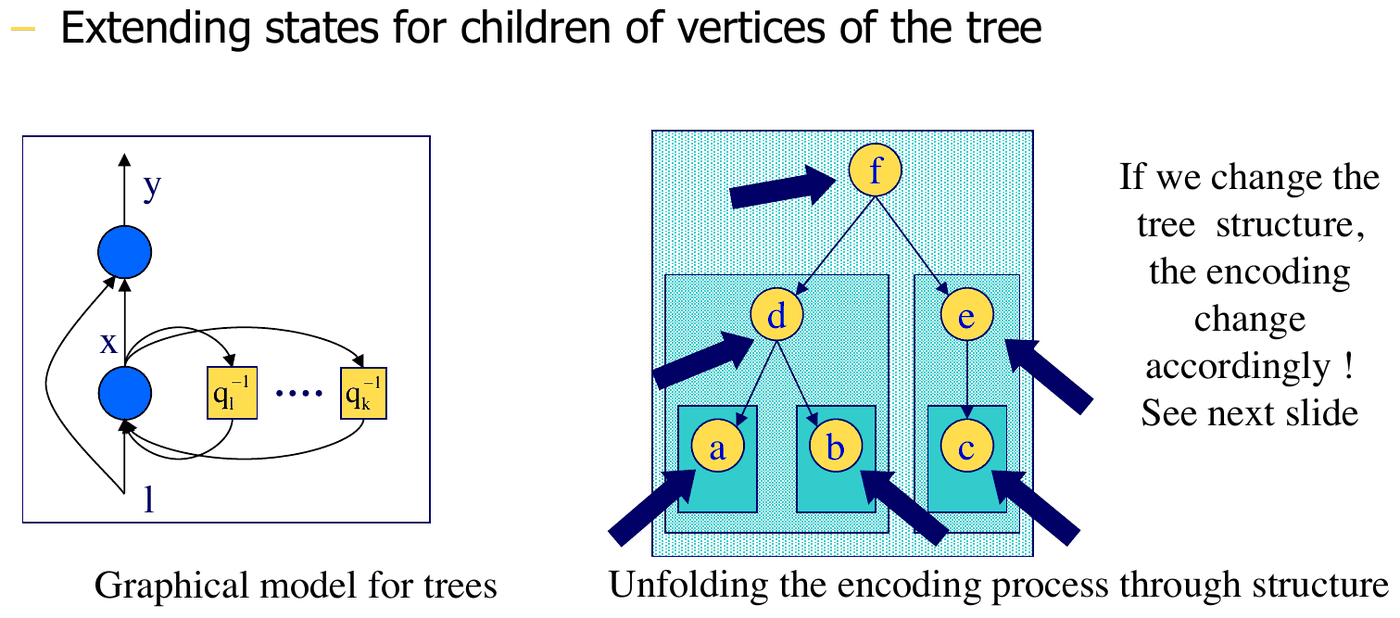
\includegraphics[width=0.74\linewidth,height=0.42\textheight,keepaspectratio]{images/20-rnn_alberi.png}
\caption{Graphical model for trees and unfolding of the encoding along
the structure: if the structure of the tree changes, the encoding
changes accordingly.}
\end{figure}

\begin{figure}[htbp]
\centering
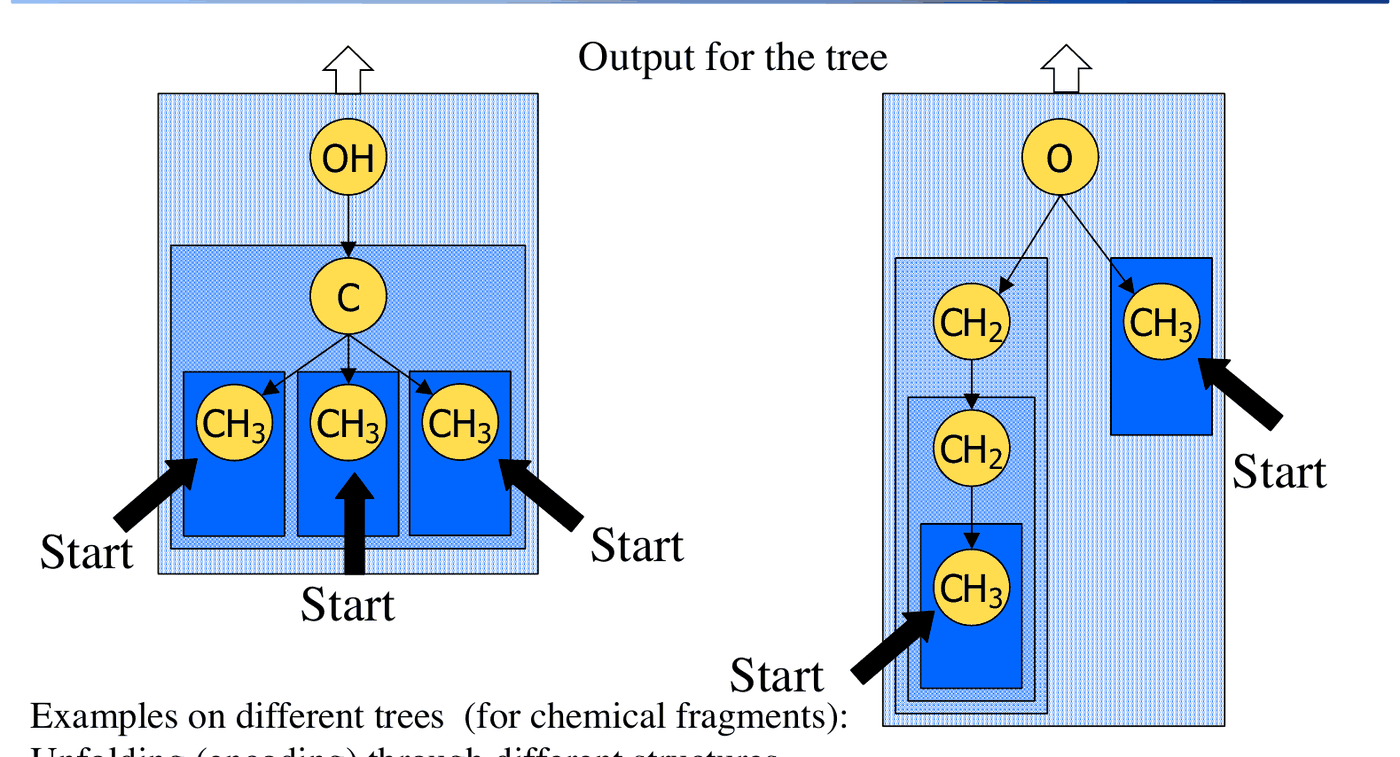
\includegraphics[width=0.74\linewidth,height=0.42\textheight,keepaspectratio]{images/20-rnn_recnn.png}
\caption{A recursive network applied to different trees (chemical
fragments): the units are the same for all the vertices of a tree and
for all the trees of the dataset (weight sharing).}
\end{figure}

\begin{boxabstract}{Summary}

RNNs add \textbf{states} and \textbf{feedback} to networks, becoming
\textbf{state transition systems} able to process variable-length
sequences. They rest on causality, stationarity and adaptivity; they
are trained by \textbf{unfolding} them in time and applying
backpropagation (BPTT, RTRL), but they suffer from the \textbf{vanishing
gradient} on long dependencies (hence LSTM and GRU). Alternatives and
developments: transformers (attention), Echo State Networks (random
reservoir + linear readout, with a Markovian bias), recursive networks
for trees and graphs.

\end{boxabstract}

\begin{boxquestion}{Possible exam questions}

\begin{itemize}
\tightlist
\item
  Why are models for sequential data needed? What is a transduction?
\item
  Difference between IDNN and RNN; why can an IDNN not count the
  ``1''s in arbitrary sequences?
\item
  Write the equation of a recurrent unit and of a Simple RNN.
\item
  What are the assumptions of causality, stationarity and adaptivity?
\item
  What is unfolding and how does it allow backpropagation to be used?
\item
  What is an Echo State Network and what is the Echo State Property?
\item
  How are RNNs extended to trees?
\end{itemize}

\end{boxquestion}
